% Chapter 2

\chapter{Radares Passivos} % Main chapter title

\label{chap:Chapter2} % For referencing the chapter elsewhere, use \ref{chap:Chapter2} 

%----------------------------------------------------------------------------------------

\section{Contextualização} \label{contextualização}
Os radares convencionais apresentam uma configuração onde são constituídos por um transmissor e um recetor, normalmente no mesmo local. Neste tipo de radares, um pulso é transmitido em forma de energia eletromagnética, e através do conhecimento do tempo levado pelo pulso a ser transmitido e recebido depois de refletido no alvo e da velocidade de propagação da luz, consegue-se determinar um valor de distância.\par 
Num radar passivo, não existe transmissão de energia eletromagnética durante o seu funcionamento. Ao invés, utiliza iluminadores de oportunidade e compara o seu sinal direto com pequenas alterações que ocorrem no campo eletromagnético por alvos em movimento de forma a detetar um alvo \parencite{Griffiths2017}.\par 
Este sistema radar pode utilizar uma grande variedade de iluminadores, desde sistemas de navegação por satélite (\textit{\gls{GNSS}}) como o \gls{GPS} ou o GLONASS, \textit{routers} de WiFi ou qualquer sistema de transmissão de frequências rádio como \textit{\gls{DVB}} ou estações de rádio. Dito isto, por forma a dimensionar o sistema para o efeito desejado, torna-se necessário uma boa compreensão das mais diversas caraterísticas dos iluminadores, como é falado mais à frente neste capítulo.\par 
Para a finalidade de deteção de alvos a grandes distâncias, os sinais mais eficazes e consequentemente mais utilizados são os que apresentam elevada potência, como transmissores de \gls{VHF} e de televisão digital em \gls{UHF}, não obstante poder-se também utilizar em certos casos outros iluminadores.\par
O cenário típico de um esquema de deteção usando um radar passivo é, como mostrado na Figura \ref{fig:esquema_pcl}, constituído por duas antenas recetoras, uma antena que recebe o sinal direto do iluminador ($S_{ref}$) e outra antena que recebe o sinal que é refletido no alvo ($S_{r}$). O sinal refletido no alvo fornece duas informações importantes para a sua deteção: o \textit{bistatic range}, ou seja, a distância ao alvo, conseguida através da diferença de tempo entre o sinal direto e o sinal refletido; e o \textit{Doppler}, que é o desvio de frequência que um alvo em movimento cria no sinal que é refletido devido à sua velocidade. Estes conceitos são discutidos mais à frente neste capitulo. \par

\begin{figure}[h]
\centering
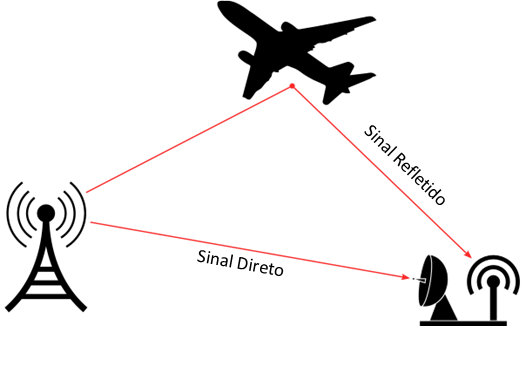
\includegraphics[scale=0.7]{chapters/ch2/assets/esquema_pcl}
\caption[Esquema Geometria Radar Passivo]{Esquema da geometria de um radar passivo}
\label{fig:esquema_pcl}
\end{figure}

O conceito do radar passivo é fazer uma relação cruzada, ou, como mais conhecido o termo, \textit{cross-correlation} entre o sinal direto e o sinal refletido em função das variáveis \textit{delay-time} que pode ser transformado em \textit{bistatic range} e o desvio de \textit{Doppler}. A \textit{cross-correlation}, de forma simples, é uma medida de similaridade entre dois sinais aplicando um atraso num deles, que neste caso, para além do atraso (\textit{delay-time}), também é feita para os diferentes \textit{Doppler}, ou seja, em duas dimensões. No entanto, na prática existem processos analíticos mais eficientes, visto que fazer a \textit{cross-correlation} a duas dimensões em tempo real torna o processo muito pesado computacionalmente.



\subsection{Geometrias Radar}
Podemos classificar os radares quanto à localização dos transmissores e recetores. O ângulo $\beta$ que estes formam, sendo o seu centro o alvo, determina o tipo de geometria \parencite{Baker2019}. Se $\beta <20^{\circ}$, o transmissor e o recetor encontram-se perto ou no mesmo sítio, então estamos perante uma geometria monostática (Figura \ref{fig:monostatic}). Quando o transmissor e recetor estão mais afastados e formam um ângulo com centro no recetor dentro dos seguintes limites, $20^{\circ}<\beta <145^{\circ}$, a geometria é bistática (Figura \ref{fig:bistatic}). Para situações particulares, em que o alvo se encontra a uma cota baixa em relação à linha imaginária que une o transmissor e o recetor ($145^{\circ}<\beta <180^{\circ}$), estamos perante uma geometria \textit{Forward Scatter} (Figura \ref{fig:fsc}).\par   

\begin{figure}[h]
\centering
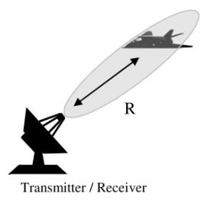
\includegraphics[scale=0.8]{chapters/ch2/assets/monostatic}
\caption[Geometria Monostática]{Geometria Monostática}
\label{fig:monostatic}
\end{figure}

\begin{figure}[h]
\centering
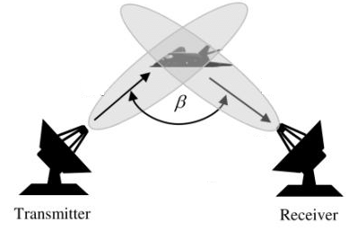
\includegraphics[scale=0.8]{chapters/ch2/assets/bistatic}
\caption[Geometria Bistática]{Geometria Bistática}
\label{fig:bistatic}
\end{figure}

\begin{figure}[h]
\centering
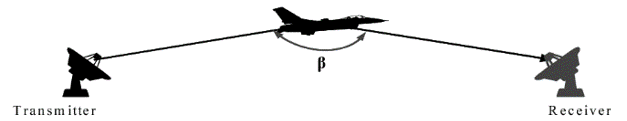
\includegraphics[scale=0.7]{chapters/ch2/assets/fsc}
\caption[Geometria \textit{Forward Scatter}]{Geometria \textit{Forward Scatter}}
\label{fig:fsc}
\end{figure}

Os radares passivos, como já discutido, têm a vantagem de não transmitirem um sinal, e ao invés usar um sinal a ser transmitido por outra fonte. Isto implica que o transmissor e o recetor não estejam no mesmo sítio nem perto, logo, quando se fala em radares passivos, assume-se uma geometria bistática.



\subsection{Alcance Bistático e \textit{Doppler}}
Como falado no ínicio deste capítulo, o alcance bistático, ou \textit{bistatic range} e o desvio de \textit{Doppler} são varáveis fundamentais para qualquer sistema radar e isso não exclui o radar passivo.\par 
O recetor bistático pode medir 3 parâmetros diferentes:
\begin{itemize}
\item A diferença em alcance entre o sinal direto e o sinal que é refletido, ou seja, o \textit{bistatic range};
\item O desvio de \textit{Doppler} do sinal recebido;
\item O ângulo $\theta_{R}$ do sinal recebido, se for usada uma antena de \textit{surveillance }direcional.
\end{itemize}

\subsubsection*{Alcance Bistático} 
Tal como representado na Figura \ref{fig:geom}, tomamos os valores $R_{T}$ como a distância do transmissor ao alvo,  $R_{R}$ como a distância do recetor ao alvo,  $\beta$ como o ângulo entre estes e com centro no alvo, e  $C$ como a distância do transmissor ao recetor, ou, \textit{Baseline}.\par


\begin{figure}[h]
\centering
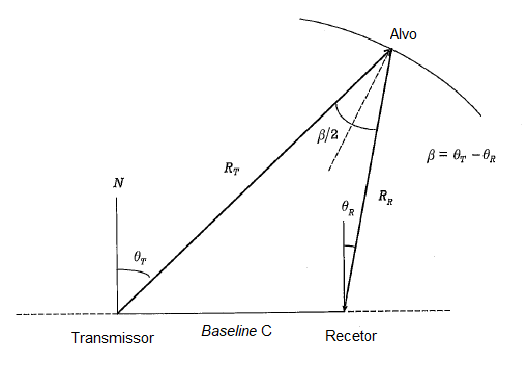
\includegraphics[scale=0.9]{chapters/ch2/assets/geom}
\caption[Parâmetros na geometria bistática]{Parâmetros na geometria bistática}
\label{fig:geom}
\end{figure}

O termo alcance bistático, ou \textit{bistatic range}, é definido em \ref{2.1}. Com este valor é possível criar elipses bistáticas (para duas dimensões) ou elipsoides bistáticos (para três dimensões) com o transmissor e o recetor como dois focos das mesmas. \par

\begin{equation} \label{2.1}
R_{T}+R_{R}-C
\end{equation}

Contudo, se a \textit{baseline} $C$ for um valor conhecido, pode-se extrair o termo \textit{range sum} $R_{T}+R_{R}$. \par
Através do conhecimento do valor de $\theta_{R}$, que é mensurável se a antena de \textit{surveillance} for direcional, a distância do alvo ao recetor é dada pela expressão \ref{2.2}.

\begin{equation} \label{2.2}
R_{R}=\dfrac{\left(  R_{T}+R_{R}\right)^{2}-C^{2}}{2\left(  R_{T}+R_{R}+C sin\theta_{R}\right)}
\end{equation}


Um dos parâmetros importantes quando se fala em alcance bistático é a \textit{range resolution}, ou seja, a resolução em alcance. Este parâmetro é definido pela capacidade de distinguir os alvos que estão muito próximos. Um bom exemplo de um sistema radar que necessite de grande \textit{range resolution} é um sistema de direção de tiro. \par 

Num radar convencional monostático, a resolução em alcance é dada por $\Delta R=c/2B$, onde c é a velocidade de propagação e B a largura de banda do sinal transmitido. No entanto, num radar passivo, a geometria é bistática, o que leva a existirem diferentes elipses bistáticas concêntricas, isto é, com centro no mesmo ponto, o que tem de ser tomado em conta na expressão que representa a \textit{range resolution}:

\begin{equation} \label{2.3}
\Delta r=\dfrac{c}{2B\left( \dfrac{cos\beta}{2}\right)}
\end{equation}

No entanto, este caso é específico para quando os dois alvos estão alinhados relativamente à bissetriz do ângulo $\beta$, como é possivel observar na figura \ref{fig:geom_varios_alvos} o exemplo dos alvos 1 e 2. Para um caso generalizado, como por exemplo o alvo 1 e o alvo 3, a expressão da \textit{bistatic range resolution} (Expressão \ref{2.4}) depende de mais um valor $\varphi$ representado na figura \ref{fig:geom_varios_alvos} como o ângulo entre o seguimento da bissetriz do ângulo $\beta$ e o segmento de reta que une o alvo 1 e o alvo 3 com centro no alvo 1. 

\begin{figure}[h]
\centering
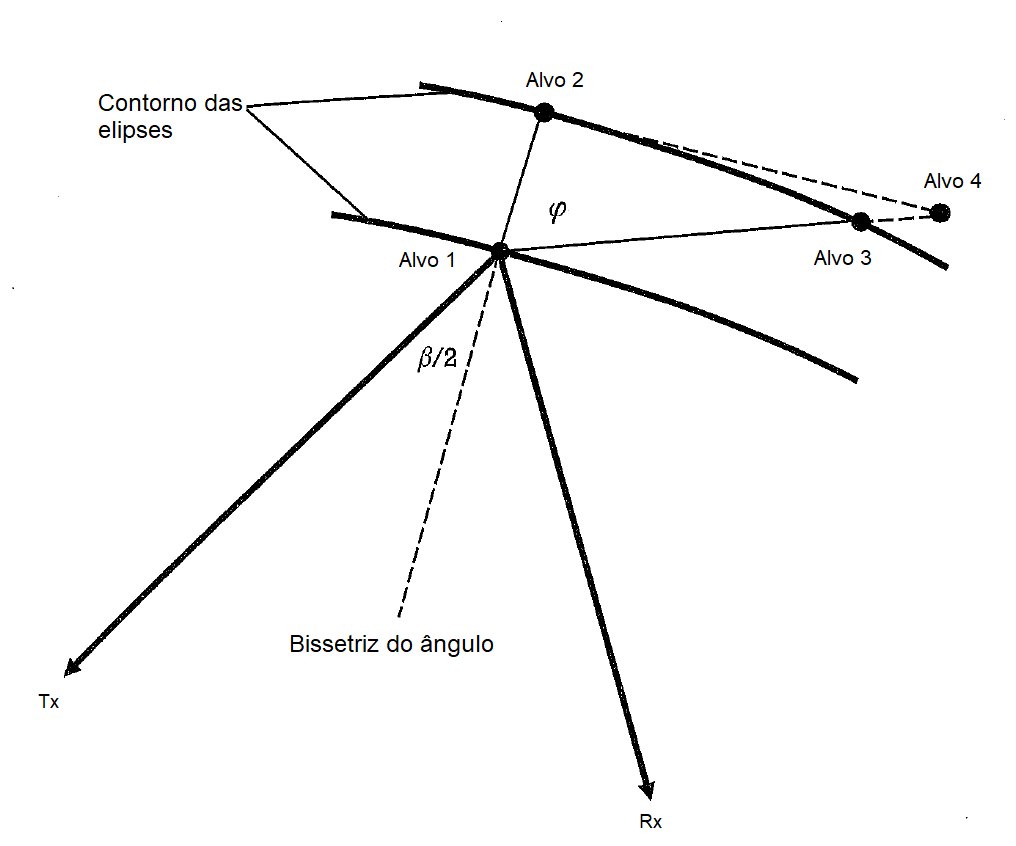
\includegraphics[scale=0.5]{chapters/ch2/assets/geom_varios_alvos}
\caption[Geometria bistática para vários alvos]{Geometria bistática para vários alvos (Adaptada da figura 2.4 \cite{Griffiths2017})}
\label{fig:geom_varios_alvos}
\end{figure}


\begin{equation} \label{2.4}
\Delta r=\dfrac{c}{\left[ 2B\left( \dfrac{cos\beta}{2}\right)\right] cos\varphi}
\end{equation}


A expressão do \textit{bistatic range resolution} permite interpretar a geometria bistática quanto à distância entre o transmissor e recetor. Da expressão \ref{2.4} conclui-se que quanto mais o ângulo $\beta$ se aproxima de um ângulo reto, o denominador tende para um valor próximo de 0, ou seja, a resolução em alcance torna-se fraca. Contudo, nesta situação estamos perante uma geometria \textit{forward scatter}, discutido no inicio deste capítulo, o que pode ser contornando usando vários recetores em locais diferentes.\par 
Para radares passivos, continuando a interpretação da expressão \ref{2.4}, os iluminadores de oportunidade mais utilizados têm pouca largura de banda $B$, o que se reflete numa resolução em alcance mais reduzida. No entanto, os sinais de DVB-T, discutidos no Capítulo \ref{chap:Chapter1}, têm uma largura de banda na ordem dos 8 MHz, o que já permite uma resolução em alcance na ordem dos 40m.

\subsubsection*{\textit{Doppler}} 
Ignorando efeitos relativisticos, o desvio de \textit{Doppler} bistático ocorre quando pelo menos um dos elementos transmissor, alvo, recetor se encontra em movimento. É definido como a taxa de variação temporal do comprimento total do caminho percorrido pelo sinal refletido, normalizado pelo comprimento de onda $\lambda$ \parencite{Willis2005}.  No caso mais comum, em que apenas o alvo se encontra em movimento, o desvio de \textit{Doppler} é dado por \parencite{Willis2005},

\begin{equation} \label{2.5}
f_{D}=\dfrac{2v}{\lambda}cos\delta cos\left( \dfrac{\beta}{2}\right) 
\end{equation}

onde $\delta$ é o ângulo formado pelo sentido do vetor velocidade $v$ e a bissetriz do ângulo $\beta$ com centro no alvo. \par

Na equação \ref{2.5}, quando $\beta =180^{\circ}$, estamos perante uma geometria \textit{forward scatter} e temos um valor de desvio de \textit{Doppler} $f_{D}=0$ para todos os ângulos de $\delta$. Quando $\beta =0^{\circ}$, fica-se reduzido a uma geometria monostática. 


A resolução de \textit{Doppler} no radar bistático é semelhante à resolução de \textit{Doppler} no radar monostático, isto porque depende do tempo de integração $T$ que é um parâmetro escolhido e indiferente à geometria do radar. Quanto maior for o tempo de integração, melhor é a resolução de \textit{Doppler}. A expressão \ref{2.6} define o requisito mínimo entre a separação dos alvos.

\begin{equation} \label{2.6}
\vert f_{a1}-f_{a2}\vert = \dfrac{1}{T}
\end{equation}

sendo que $f_{a1}$ e $f_{a2}$ são os desvios de \textit{Doppler} para cada alvo, definidos em \ref{2.5}. Substituindo as equações dos alvos em \ref{2.5} na equação \ref{2.6}, e resolvendo em ordem a $\Delta v$, ou seja, a diferença entre os dois vetores velocidade projetados na bissetriz do ângulo $\beta$ ($\Delta v=\left( v_{1}cos\delta_{1}-v_{2}cos\delta_{2}\right) $), vem,

\begin{equation} \label{2.7}
\Delta v = \dfrac{\lambda}{2T\cdot cos\left( \beta /2\right) }
\end{equation}

Com esta expressão, assumimos que os alvos partilham a mesma bissetriz, o que na realidade é pouco provável. No entanto, esta restrição pode ser ignorada, se,
\begin{enumerate}
	\item A separação entre os alvos não for suficiente para permitir resolução em \textit{range};
	\item O ângulo entre as bissetrizes dos dois alvos é pequeno.
\end{enumerate}


\subsection{Processamento de Sinal}
Como falado em \ref{contextualização}, o conceito do radar passivo é fazer uma \textit{cross-correlation} entre o sinal direto e o refletido. O problema está no facto de ser computacionalmente muito pesado fazer uma \textit{\gls{2D-CCF}}, sendo necessário a utilização de algoritmos mais eficientes para o cálculo da mesma.\par
O processamento de sinal num radar passivo pode ser, resumidamente, enumerado em oito pontos:
\begin{enumerate}
	\item Receção e reconstrução do sinal direto (\textit{reference signal}$s_{ref}$)
	\item Receção do \textit{surveillance signal} ($s_{r}$))
	\item \textit{Cross-correlation} do $s_{ref}$ e $s_{r}$
	\item Integração de produtos da correlação (FFT)
	\item Filtragem de \textit{clutter}
	\item Deteção de alvos e seguimento no domínio \textit{range/Doppler}
	\item Processamento no plano Cartesiano
	\item Seguimento no plano Cartesiano
\end{enumerate}

\subsubsection*{Equivalência entre um filtro adaptado e \textit{cross-correlation}}

Para \textit{Software Defined Radios}, a implementação de um filtro adaptado pode ser feita através do cálculo de uma \textit{cross-correlation} \parencite{Martorella}. Considerando $s_{0}(t)$ o sinal de saída do filtro adaptado e $h_{MF}(t)$ a resposta do filtro vem, 

\begin{equation} \label{2.8}
s_{0}\left( t\right) =s_{R}\left( t\right)\otimes h_{MF}\left( t\right) =\int s_{R}\left( \tau\right)s_{ref}^{\ast}\left(\tau -t\right)d\tau
\end{equation}

A equação \ref{2.8} mostra que usando um filtro adaptado obtemos um sinal de saída igual ao fazer uma \textit{cross-correlation} entre o $s_{R}$ e $s_{ref}$.\par 

Ao implementar uma \textit{cross-correlation} como mostrado em \ref{2.8}, não se toma em conta o desvio de \textit{Doppler}, visto que se faz a \textit{cross-correlation} apenas numa dimensão. Para se entrar com o desvio de \textit{Doppler} tem de se extender a \gls{2D-CCF},

\begin{equation} \label{2.9}
CCF\left( \tau,\nu\right) =\int s_{R}\left( \tau\right)s_{ref}^{\ast}\left(\tau -t\right)e^{-2\pi j\nu t}d\tau
\end{equation}

onde $\nu$ representa o desvio de \textit{Doppler} que é definido pela \textit{cross-correlation} entre o $s_{R}$ e $s_{ref}$ compensada com o \textit{Doppler shift}.\par
Como o \textit{delay-time} $\tau$ pode ser transformado em \textit{bistatic range}, a \gls{2D-CCF} pode ser representada num \textit{bistatic range-Doppler map}, através da equação \ref{2.10} que representa a \gls{2D-CCF} numéricamente visto que os sinais têm de ser digitalizados com uma certa frequência de amostragem.

\begin{equation} \label{2.10}
CCF\left(l,m\right) =\sum_{n=0}^{N-1} s_{R}\left( n\right)s_{ref}^{\ast}\left(n -l\right)e^{-2\pi j\dfrac{mn}{N}}
\end{equation}

onde $n$ representa o tempo, $l$ o \textit{delay-time}, $m$ o desvio de \textit{Doppler} e $N$ o número total de amostras que depende do \gls{CPI},

\begin{equation} \label{2.11}
N=\dfrac{CPI}{T_{s}}=CPI\cdot F_{s}
\end{equation}

\subsubsection*{Eficiência do cálculo da \gls{2D-CCF}}
De modo a ter um cálculo da \gls{2D-CCF} mais eficiente, há duas condições principais a referir:
\begin{itemize}
\item Cumprir com o teorema de \textit{Nyquist}, ou seja, garantir que a frequência de amostragem é superior ou igual à largura de banda ($F_{s}\geq B$); 
\item Ter um \gls{CPI} longo de forma a obter maior ganho de integração e consequentemente melhor relação sinal-ruído.
\end{itemize}
\par
No entanto, o cálculo de uma \gls{2D-CCF} é computacionalmente muito pesado, e isto pode ser demonstrado com um pequeno exemplo: Para uma largura de banda $B=10MHz$, um $CPI=1s$ e um número de \textit{range bins} e de \textit{doppler bins} igual a 1000 cada, implica um número de multiplicações muito elevado ($10000000\cdot 1\cdot 1000\cdot 1000=10000000000$ cálculos).\par
Para solucionar este problemas existem várias soluções numéricas, como \textit{Correlation FFT}, \textit{Direct FFT} e \textit{Batches Algorithm} \parencite{Martorella}.

\subsubsection*{\textit{Correlation FFT}}
A \textit{Correlation FFT} pode ser obtida através da equação \ref{2.10} mudando o exponencial de posição como representado na eq. \ref{2.12}, de modo a obter uma nova expressão que pode ser calculada como uma \textit{cross-correlation} a uma dimensão com uma compensação de \textit{Doppler}, ou seja, \textit{Doppler bin} ($m$), a \textit{\gls{CCF}} é a \textit{cross-correlation} entre o \textit{reference signal} $S_{ref}$ e o sinal direto com um \textit{Doppler shift}.

\begin{equation} \label{2.12}
CCF\left(l,m\right) =\sum_{n=0}^{N-1} s_{R}\left( n\right)e^{-2\pi j\dfrac{mn}{N}}s_{ref}^{\ast}\left(n -l\right)
\end{equation}

Substituindo $s_{R}\left( n\right)e^{-2\pi j\dfrac{mn}{N}}$ por $s_{R}(n,m)$ vem,

\begin{equation} \label{2.13}
CCF\left(l,m\right) =\sum_{n=0}^{N-1} s_{R}\left( n,m\right) s_{ref}^{\ast}\left(n -l\right)
\end{equation}

Com isto, e sabendo que as \textit{cross-correlations} são calculadas mais eficientemente no domínio de \textit{Fourier}, vem,

\begin{equation} \label{2.14}
CCF\left(l,m\right) = IDFT\left[ S_{R}\left( k,m\right)S_{ref}^{\ast}\left(k\right)\right] 
\end{equation}

com 

\begin{equation} \label{2.15}
S_{R}\left( k,m\right)  = DFT\left[ s_{R}\left( n,m\right) \right] 
\end{equation}

\begin{equation} \label{2.16}
S_{ref}\left( k\right)  = DFT\left[ s_{ref}\left( n\right) \right] 
\end{equation}

A \gls{DFT} da versão do sinal direto com \textit{Doppler shift} pode ser calculada apenas uma vez porque a variável $m$ apenas causa um desvio circular.
Com isto, pode-se tirar algumas conclusões \parencite{Martorella}:
\begin{itemize}
\item Apenas é necessário calcular a \textit{\gls{DFT}} de $s_{R}\left( n,m\right)$ uma vez para $m=0$, visto que para outros valores de $m$ podem ser obtidos com um desvio;
\item Em cada iteração, são calculadas N multiplicações complexas e uma \textit{\gls{IDFT}}.
\end{itemize}

Com isto, concluímos que quanto menos \textit{doppler bins} existirem em relação aos \textit{range bins}, mais eficiente será o cálculo. Este pode ser expressado através da seguinte função de complexidade:

\begin{equation} \label{2.17}
O_{CF}=2Nlog_{2}(N)+N_{f}[N+Nlog_{2}(N)]
\end{equation}

onde,
$N_{f}$: "Número de doppler bins"

\subsubsection*{\textit{Direct FFT}}
Por outro lado, a \textit{Direct FFT} é um método que, tal como a \textit{Correlation FFT} deriva da interpretação da equação \ref{2.10} mas, para cada \textit{time bin} $l$, a \textit{\gls{CCF}} é a \gls{DFT} do produto do sinal recebido com a versão conjugada com \textit{delay} do \textit{reference signal} $S_{ref}$.

\begin{equation} \label{2.18}
CCF\left(l,m\right) = DFT\left[ S_{R}\left( n\right)S_{ref}^{\ast}\left(n-l\right)\right] 
\end{equation}

Da interpretação da equação \ref{2.18} conclui-se que, para cada iteração, são calculadas N multiplicações complexas e u,a \gls{DFT}. A sua função de complexidade pode ser expressa através da expressão \ref{2.19}:


\begin{equation} \label{2.17}
O_{DF}=N_{\tau}[N+Nlog_{2}(N)]
\end{equation}

onde,
$N_{\tau}$: "Número de range bins"

Ao contrário da \textit{correlation FFT}, tal como se pode observar na função de complexidade, a eficiência deste método é dependente do $N_{\tau}$. Isto é, o número de iterações feitas neste método está diretamente relacionado com o número de \textit{range cells}: quanto maior for o número de \textit{range cells} do mapa \textit{range-Doppler}, menos eficiente é este método.\par

\begin{figure}[h]
\centering
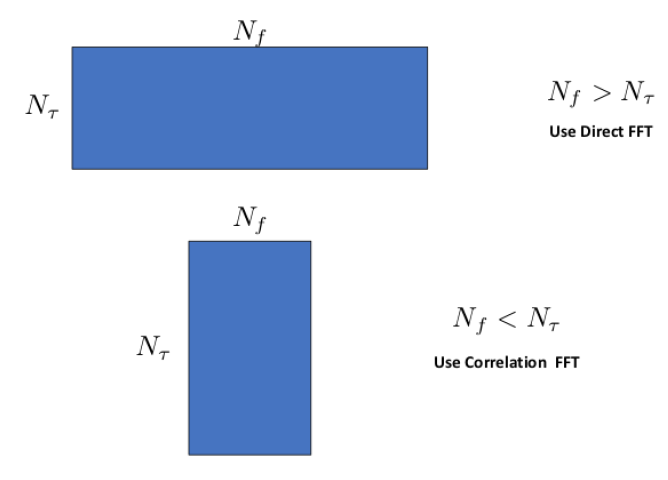
\includegraphics[scale=0.6]{chapters/ch2/assets/cfft_vs_dfft}
\caption[Correlation FFT vs Direct FFT]{\textit{Correlation FFT vs Direct FFT} (Figura 2.4 \cite{Martorella})}
\label{fig:cfft_vs_dfft}
\end{figure}

A figura \ref{fig:cfft_vs_dfft} representa de uma forma ilustrativa quando usar a \textit{Direct FFT} ou \textit{Correlation FFT} de acordo com a relação de \textit{Doppler cells} e \textit{range cells} no mapa de \textit{range-Doppler}. Se existirem mais \textit{Doppler cells} a \textit{Direct FFT} é mais eficiente, enquanto se o contrário se verificar, a \textit{Correlation FFT} torna-se mais eficiente.

\subsubsection*{\textit{Batches algorithm}}





\subsection{Supressão do Sinal Direto}




\subsection{Previsão de \textit{Performance}}



\subsection{Formação de Imagem}

